              
% --------------------------------------------------------------
% This is all preamble stuff that you don't have to worry about.
% Head down to where it says "Start here"
% --------------------------------------------------------------
 
\documentclass[12pt]{article}
 
\usepackage[margin=1in]{geometry} 
\usepackage{amsmath,amsthm,amssymb}
\usepackage{url}
\usepackage{graphicx}
\usepackage{float}
\usepackage{paralist}
\setlength{\parindent}{0mm}
\newcommand{\N}{\mathbb{N}}
\newcommand{\Z}{\mathbb{Z}}
 
\newenvironment{theorem}[2][Theorem]{\begin{trivlist}
\item[\hskip \labelsep {\bfseries #1}\hskip \labelsep {\bfseries #2.}]}{\end{trivlist}}
\newenvironment{lemma}[2][Lemma]{\begin{trivlist}
\item[\hskip \labelsep {\bfseries #1}\hskip \labelsep {\bfseries #2.}]}{\end{trivlist}}
\newenvironment{exercise}[2][Exercise]{\begin{trivlist}
\item[\hskip \labelsep {\bfseries #1}\hskip \labelsep {\bfseries #2.}]}{\end{trivlist}}
\newenvironment{reflection}[2][Reflection]{\begin{trivlist}
\item[\hskip \labelsep {\bfseries #1}\hskip \labelsep {\bfseries #2.}]}{\end{trivlist}}
\newenvironment{proposition}[2][Proposition]{\begin{trivlist}
\item[\hskip \labelsep {\bfseries #1}\hskip \labelsep {\bfseries #2.}]}{\end{trivlist}}
\newenvironment{corollary}[2][Corollary]{\begin{trivlist}
\item[\hskip \labelsep {\bfseries #1}\hskip \labelsep {\bfseries #2.}]}{\end{trivlist}}
 
\begin{document}
 
% --------------------------------------------------------------
%                         Start here
% --------------------------------------------------------------
 
%\renewcommand{\qedsymbol}{\filledbox}
 
\title{\bf Fortran Modernisation Workshop \\ Exercises}
\author{F. Spiga, F. Chami and W. Miah}
 
\maketitle

This exercise will involve modernising a legacy Fortran code\footnote{\url{https://people.sc.fsu.edu/~jburkardt/f77_src/fd1d_heat_explicit/fd1d_heat_explicit.html}} which is written 
in Fortran 77 to modern Fortran. The code solves the one dimensional heat
diffusion equation:
\begin{equation} \label{fd1hd}
\frac{\partial{\bf H}}{\partial t} - K\frac{\partial^{2}{\bf H}}{\partial x^{2}} = f(x)
\end{equation}
where $K$ is the heat coefficient. Equation~(\ref{fd1hd}) describes the distribution of heat 
between $x_{\text{min}}$ and $x_{\text{max}}$ and uses the following explicit finite difference 
scheme to integrate in time:
\begin{align}
{\bf H}^{(n+1)}_{i} & = {\bf H}^{(n)}_{i} + \text{CFL}\big\{{\bf H}^{(n)}_{i-1}-2{\bf H}^{(n)}_{i} +
                      {\bf H}^{(n)}_{i+1}\big\} + \Delta t f(x_{i}) \label{fd} \\
            \text{where CFL} & = k\frac{\Delta t}{\Delta x^{2}} \label{cfl}
\end{align}
Equation~(\ref{cfl}) is known as the Courant-Friedrichs-Lewy coefficient which must satisfy
the condition $\text{CFL} \le 0.5$ for the scheme~(\ref{fd}) to be stable. Don't worry if you do 
not know what all this means - the focus of the exercise is on Fortran programming and not
Maths. \\

The exercises are split into two parts: one set for the first day and a second
set for the second day. Obtain the exercises by using the commands:
\begin{verbatim}
cp /usr/local/src/fmw_exercise.tar.gz $HOME
cd $HOME
tar -zxvf fmw_exercise.tar.gz
\end{verbatim}
which will extract the exercises to the \texttt{fmw\_exercise/} directory. Change into the 
\texttt{fmw\_exercise/} directory:
\begin{verbatim}
git config --global user.name "firstname lastname"
git config --global user.email firstname.lastname@address.com
cd fmw_exercise
git init
git add .
git commit -m "initial version"
\end{verbatim}
The Git commands will version control your code so you can see its revision history. Git will
be covered in the second session. \\

Day one exercises will include modernising an existing Fortran 77 code. Day two exercises will involve the 
following topics:
\begin{enumerate}
\item Makefiles for Fortran codes;
\item Git source code version control system;
\item Doxygen code documentation tool for Fortran codes;
\item NetCDF file format for arrays;
\item In-memory visualisation using PLplot
\item Unit testing with pFUnit.
\end{enumerate}
\newpage
\subsection*{Day One Exercises}
\setdefaultleftmargin{0pt}{}{}{}{}{}
\begin{enumerate}
\item Create a module \texttt{Types\_mod} and put it in the file \texttt{Types\_mod.f90} which 
contains the following numeric data types:
\begin{verbatim}
use, intrinsic :: iso_fortran_env
integer, parameter :: SP = REAL32
integer, parameter :: DP = REAL64
integer, parameter :: SI = INT32
integer, parameter :: DI = INT64
\end{verbatim}
using the following module template: 
\begin{verbatim}
module Types_mod
   use, intrinsic :: iso_fortran_env

   implicit none

   public :: SP

   integer, parameter :: SP = REAL32
contains

end module Types_mod
\end{verbatim}
The above\label{mod:temp}
\item In the main program code (file \texttt{fd1d\_heat\_explicit.f90} including all functions and subroutines), include the double colon after the variable type and before 
the variable name, e.g. from \texttt{double precision a} to \texttt{double precision :: a}
\item In the main program code, include the line \texttt{use Types\_mod} just before
the \texttt{implicit none} statement. This will allow you to use the constants declared in the
\texttt{Types\_mod} Fortran module
\item In the main program code, use the \texttt{kind} keyword in variable declarations, e.g.
from \texttt{double precision} to \texttt{real(kind=DP)} and \texttt{integer} to 
\texttt{integer(kind=SI)}
\item In the main program code, change how parameters are declared, e.g. from 
\texttt{parameter ( T\_NUM = 201 )} to \texttt{integer(kind=SI), parameter :: T\_NUM = 201} and the
same for the variable \texttt{X\_NUM}
\item In the main program code, change how constants are used, e.g. from \texttt{0.0D+00} to 
\texttt{0.0\_DP}
\item In the functions and subroutines, use the \texttt{intent} keyword for dummy arguments
\item In the main program code, use dynamic memory allocation for the arrays \texttt{h(1:X\_NUM)}, 
\texttt{h\_new(1:X\_NUM)}, \texttt{hmat(1:X\_NUM,1:T\_NUM)}, \texttt{t(1:T\_NUM)}, \texttt{x(1:X\_NUM)}. Check
the status of the dynamic memory allocation\label{dyn:memory}
\item At the end of the main program code, deallocate the arrays declared in step~\ref{dyn:memory}
\item In the functions and subroutines, remove the size of the array and use assumed shaped
arrays as dummy arguments:
\begin{itemize}
\item For the function \texttt{func( j, x\_num, x )} remove the \texttt{x\_num} argument and
replace the argument declaration to \texttt{real(kind=DP), dimension(:) :: x}. Make sure
invocations of \texttt{func( )} reflect this change
\item For the function \texttt{fd1d\_heat\_explicit( )} remove the \texttt{x\_num} argument
and ensure all arrays are declared as assumed shaped arrays. Use the automatic arrays feature in Fortran
to declare the array \texttt{f(:)} as \texttt{real(kind=DP) :: f(size(x))}
\item For the function \texttt{r8mat\_write( )} remove the arguments \texttt{m} and \texttt{n} and assign them
to \texttt{size( table(:,:), 1 )} and \texttt{size( table(:,:), 2 )}, respectively. Declare the argument \texttt{table(:,:)}
as an assumed shaped array
\item For the function \texttt{r8vec\_linspace( )} remove the argument \texttt{n} and declare the argument \texttt{a(:)} as
an assumed shaped array
\item For the function \texttt{r8vec\_write( )} remove the argument \texttt{n} and declared the argument \texttt{x(:)} as
an assumed shaped array
\end{itemize}
Use the \texttt{size( )} intrinsic function to get array dimensions. 
\item In the main program code, use the modern string declaration statement. For dummy argument
declaration:
\begin{verbatim}
character * ( * ) string    ! to
character(len=*) :: string
\end{verbatim}
For string declarations:
\begin{verbatim}
character * ( 30 ) :: string             ! to
character(len=30)  :: string
\end{verbatim}
\item In the main program code, use symbolic relational operators \texttt{<, <=, /=, ==, >=, >}
instead of \texttt{.lt., .le., .ne., .eq., .ge., gt.}
\item Compile both the main program and the created Fortran module:
\begin{verbatim}
gfortran -c Types_mod.f90
gfortran -c -I. fd1d_heat_explicit.f90
gfortran fd1d_heat_explicit.o Types_mod.o -o fd1d_heat_explicit.exe
./fd1d_heat_explicit.exe
\end{verbatim}
\item To test whether your code runs correctly execute:
\begin{verbatim}
diff h_test01.txt h_test01.txt_bak
\end{verbatim}
If the command outputs difference, then the refactoring introduced a bug.
\item Type \texttt{git diff fd1d\_heat\_explicit.f90} to see the refactored code. Stage and commit
the changes by typing: 
\begin{verbatim}
git add fd1d_heat_explicit.f90
git add Types_mod.f90
git commit -m "refactored Fortran 77 into modern Fortran"
\end{verbatim}
\item[] The following exercises will further modularise the code and use the module template in
  question~\ref{mod:temp} for creating additional modules.
\item Create a module \texttt{RHS\_mod} and put it in the file \texttt{RHS\_mod.f90} and put the 
Fortran function \texttt{func()} into \texttt{RHS\_mod} and declare it public. In the main program code, 
insert the line \texttt{use RHS\_mod} 
\item Create a module \texttt{CFL\_mod} and put it in the file \texttt{CFL\_mod.f90} and put the
  Fortran function \texttt{fd1d\_heat\_explicit\_cfl( )} into \texttt{CFL\_mod} and declare it
  public. In the main program
code, insert the line \texttt{use CFL\_mod}
\item Create a module \texttt{IO\_mod} and put it in the file \texttt{IO\_mod.f90} and put
  the Fortran functions \texttt{r8mat\_write( )}, \texttt{r8vec\_linspace( )} and \texttt{r8vec\_write( )}
  into \texttt{IO\_mod} and declare them public. In the main program code, insert the line \texttt{use IO\_mod}
\item Create a module \texttt{Solver\_mod} and put it in the file \texttt{Solver\_mod.f90} and put the
  Fortran function \texttt{fd1d\_heat\_explicit( )} into \texttt{Sover\_mod} and declare it public. In the main
  program code, insert the line \texttt{use Solver\_mod}
\item Compile the recently created modules:
\begin{verbatim}
gfortran -c RHS_mod.f90
gfortran -c CFL_mod.f90
gfortran -c IO_mod.f90
gfortran -c Solver_mod.f90
gfortran -c -I. fd1d_heat_explicit.f90
gfortran fd1d_heat_explicit.o Types_mod.o RHS_mod.o CFL_mod.o IO_mod.o \
         Solver_mod.o -o fd1d_heat_explicit.exe
./fd1d_heat_explicit.exe
\end{verbatim}
\item To test whether your code runs correctly execute:
\begin{verbatim}
diff h_test01.txt h_test01.txt_bak
\end{verbatim}
If the command outputs difference, then the refactoring introduced a bug.
\item Add the newly created module files into Git and stage the changed main program for a
another Git commit:
\begin{verbatim}
git add RHS_mod.f90 CFL_mod.f90 IO_mod.f90 Solver_mod.f90
git add fd1d_heat_explicit.f90
git commit -m "modularised RHS, CFL, IO and Solver"
\end{verbatim}
%
\end{enumerate}
\newpage
\subsection*{Day Two Exercises}
\begin{enumerate}
\item Write a Makefile for the Fortran code produced on day one in the same directory as the source
  code using the dependency graph in Figure~\ref{make_depend:eps}

\begin{figure}[H]
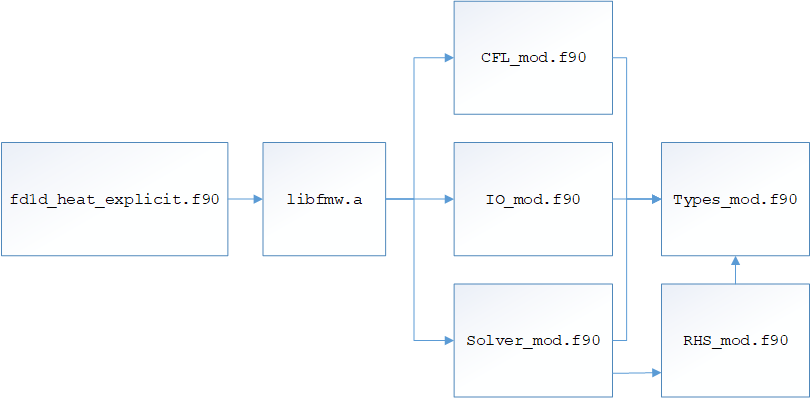
\includegraphics[width=\linewidth]{make_depend.png}
\caption{Dependency graph for Makefile}
\label{make_depend:eps}
\end{figure}
\item Add a \texttt{clean} target which cleans the build:
\begin{verbatim}
.PHONY: clean

clean:
        rm -f *.mod *.o *.png fd1d_heat_explicit.exe
\end{verbatim}
Remember to precede the commands with the tab
\item Create a static library containing all the module object files:
\begin{verbatim}
ar rcs libfmw.a CFL_mod.o IO_mod.o RHS_mod.o Solver_mod.o Types_mod.o
\end{verbatim}
In the Makefile, use the static library \texttt{libfmw.a} in the link stage to create the final executable
\begin{enumerate}
\item After creating your Makefile, type \texttt{make -n} to see what commands will be executed without executing
your commands which is useful for debugging
\item Then type \texttt{make} to build your code 
\item After creating the Makefile, add it to git using \texttt{git add Makefile}
\item Use the Linux command: 
\begin{verbatim}
nm libfmw.a
\end{verbatim}
which shows the symbols listed in the library just created. The symbol type field shows \texttt{T} for the symbol being 
defined in the library and \texttt{U} being undefined but being called by the library. 
\end{enumerate}
\item This task will cover Git in a bit more detail.
\begin{enumerate}
\item Type \texttt{git status} which will list the status of all the files. Notice that the object 
files (\texttt{*.o}), Fortran module files (\texttt{*.mod}) and executable files (\texttt{*.exe}) are listed as 
untracked files. These files need not be version controlled as they can be recreated
\item Create the file \texttt{.gitignore} in the source code directory. This configuration file will 
specify which files to not version control, e.g. object files, executable files or any file that can
be recreated. Add the following extensions in the ignore file:
\begin{verbatim}
*.o
*.mod
*.exe
*.nc
*.dat
doxygen
\end{verbatim}
\item The \texttt{.gitignore} file also needs to be version controlled using \texttt{git add .gitignore}
\item Browse the commit history of all the Fortran files created using \texttt{git log}
\end{enumerate}
\item To create a Doxygen template configuration, type \texttt{doxygen -g fortran.dxg} in the same
directory where the code resides. Then open the file \texttt{fortran.dxg} in any editor and set the 
following variables:
\begin{center}
\begin{tabular}{| c | c |} \hline
{\bf Description} & {\bf Variable and value} \\ \hline
Free text for project name & \texttt{PROJECT\_NAME = "Fortran Workshop"} \\ \hline
Free text for project description & \texttt{PROJECT\_BRIEF = "Fortran Workshop"} \\ \hline
Output directory for doxygen files & \texttt{OUTPUT\_DIRECTORY = doxygen} \\ \hline
Configuring Doxygen for Fortran & \texttt{OPTIMIZE\_FOR\_FORTRAN = YES} \\ \hline
Input directory where code resides & \texttt{INPUT = .} \\ \hline
Fortran code file extension & \texttt{FILE\_PATTERNS = *.f90} \\ \hline
Generate HTML reports & \texttt{GENERATE\_HTML = YES} \\ \hline
Using Graphvis for generating call graphs & \texttt{HAVE\_DOT = YES} \\ \hline
Generate call graph & \texttt{CALL\_GRAPH = YES} \\ \hline
Generate caller graph & \texttt{CALLER\_GRAPH = NO} \\ \hline
Extract all documentation & \texttt{EXTRACT\_ALL = YES} \\ \hline
Extract private members of class & \texttt{EXTRACT\_PRIVATE = YES} \\ \hline
Extract static members of file & \texttt{EXTRACT\_STATIC = YES} \\ \hline
List source code of file & \texttt{SOURCE\_BROWSER = YES} \\ \hline
Use free form Fortran & \texttt{EXTENSION\_MAPPING = f90=FortranFree} \\ \hline
\end{tabular}
\end{center}
Run the Doxygen command \texttt{doxygen fortran.dxg} and then load the file \newline
\texttt{doxygen/html/index.html} in any Web browser to browse the source code documentation.
\begin{enumerate}
\item Click on \texttt{Files} $\rightarrow$ \texttt{fd1d\_heat\_explicit.f90} which should display a call graph;
\item Click on \texttt{Got to the source code of this file} to see the source code of the main program code;
\item Click on \texttt{Files} $\rightarrow$ \texttt{Types\_mod.f90} $\rightarrow$ \texttt{types\_mod} to see
the public constants in the module
\item Have a browse around the other links to familiarise yourself with Doxygen;
\item Then add the Doxygen configuration file to Git by typing \texttt{git add fortran.dxg}
\item On line 1 of the file \texttt{fd1d\_heat\_explicit.f90} add the following Doxygen tags:
\begin{verbatim}
!> @author
!> <Your name>, <your affiliation>
!> @brief 
!> Solves the one dimensional heat diffusion equation
!> \f$ \frac{\partial{\bf H}}{\partial t} 
!>       - K\frac{\partial^{2}{\bf H}}{\partial x^{2}} = f(x) \f$
\end{verbatim}
\item On line 1 of the module file \texttt{CFL\_mod.f90} add the following Doxygen tags:
\begin{verbatim}
!> @author
!> <Your name>, <your affiliation>
!> @brief
!> calculates the CFL number
\end{verbatim}
In the same module file and before the subroutine \texttt{fd1d\_heat\_explicit\_cfl( )} is defined add
the following Doxygen content:
\begin{verbatim}
!> @author
!> <Your name>, <your affiliation>
!> @brief
!> calculates the CFL number
!> @param[in] k heat constant
!> @param[in] t_num number of intervals in t-axis
!> @param[in] t_min lower bound of t-axis
!> @param[in] t_max upper bound of t-axis
!> @param[in] x_num number of intervals in x-axis
!> @param[in] x_min lower bound of x-axis
!> @param[in] x_max upper bound of x-axis
!> @param[inout] cfl calculated CFL number
\end{verbatim}
\item Rerun the Doxygen command \texttt{doxygen fortran.dxg}
\item Refresh your browser and click on \texttt{Files} $\rightarrow$ \texttt{fd1d\_heat\_explicit.f90} and you
should now see the LaTeX heat diffusion equation with the description and author
\item Click on \texttt{Files} $\rightarrow$ \texttt{CFL\_mod.f90} $\rightarrow$ \texttt{More...} and you 
should now see the module author, subroutine author and description. In addition, you should see the subroutine
dummy arguments with their description
\item In your own time and after the workshop has ended do the same for the remaining module files 
(\texttt{IO\_mod.f90}, \texttt{RHS\_mod.f90}, \texttt{Solver\_mod.f90}, \texttt{Types\_mod.f90})
\item Type \texttt{git add fd1d\_heat\_explicit.f90 CFL\_mod.f90} to stage the changes and then 
\texttt{git commit -m "added Doxygen tokens in source code"}
\end{enumerate}
\item The following exercises will involve using the NetCDF API by writing the
  \texttt{x(:)}, \texttt{t(:)} and \texttt{hmat(:, :)} varaibles in one file including meta-data. 
Please refer to the NetCDF documentation at~\url{http://www.nag.co.uk/market/training/fortran-workshop/netcdf-f90.pdf} 
for the details of the API. Use the following process when creating NetCDF files for writing:
\begin{itemize}
\item\texttt{NF90\_CREATE( )} to create the file and enter define mode
\item\texttt{NF90\_DEF\_DIM( )} to create the $x$ and $t$ dimensions
\item\texttt{NF90\_DEF\_VAR( )} to create the \texttt{x(:)} (variable name {\em x-range}), \texttt{t(:)} (variable name
  {\em t-range}) and \texttt{table(:, :)} (variable name {\em solution}) variables
\item\texttt{NF90\_PUT\_ATT( )} to put global and dimension attributes
\item\texttt{NF90\_ENDDEF( )} to end define mode and to enter data mode
\item\texttt{NF90\_PUT\_VAR( )} to write the data to the file
\item\texttt{NF90\_CLOSE( )} to close the file
\end{itemize}
\begin{enumerate}
\item Open the file \texttt{IO\_mod.f90} and add the line \texttt{use netcdf}
\item Open the main program code \texttt{fd1d\_heat\_explicit.f90} and pass the arguments \texttt{x(:)} and
  \texttt{t(:)} into the subroutine call \texttt{r8mat\_write( )} and change the file name from \texttt{h\_test01.txt}
  to \texttt{h\_test01.nc} - the file extension \texttt{.nc} is used to denote NetCDF files
\item Comment out the two \texttt{r8vec\_write( )} subroutine calls
\item Edit the subroutine \texttt{r8mat\_write} and add the dummy arguments:
\begin{verbatim}
real(kind=DP), dimension(:), intent(in) :: x
real(kind=DP), dimension(:), intent(in) :: t
\end{verbatim}
\item When in define mode, add the following meta data using \texttt{NF90\_GLOBAL} for \texttt{varid} argument:
  \begin{enumerate}
  \item\texttt{"purpose" = "Fortran workshop"}
  \item\texttt{"name" = "Your name"}
  \item\texttt{"institution" = "Your university"} 
  \end{enumerate}
\item In the subroutine \texttt{r8mat\_write( )} write the one-dimensional arrays \texttt{x(:)} and \texttt{t(:)} and the
  two-dimensional array \texttt{table(:, :)} into a NetCDF file
\item To compile the remember to add the line \texttt{-I/usr/lib64/gfortran/modules} in your
  Makefile which is the NetCDF Fortran module file directory on Fedora Linux. This might be
  different for your system
\item To do the final link, remember to add the link line \texttt{-L/usr/lib64 -lnetcdff -lnetcdf}
  which is where the Fortran NetCDF wrapper resides on Fedora Linux. This might be different
  for your system
\item Once your code completes, you can view the contents of the NetCDF file using \texttt{ncdump h\_test01.nc | less}
\item To verify whether your code works correctly, compare the created NetCDF file with the correct NetCDF file:
\begin{verbatim}
ncdiff -O h_test01.nc h_test01.nc.valid diff.nc
ncdump diff.nc | less
\end{verbatim}
The second command should show all zero values for the \texttt{x-range}, \texttt{t-range} and \texttt{solution} NetCDF
variables, namely that~(\ref{test:eqn}) holds:
\begin{equation} \label{test:eqn}
||{\bf u}_{\texttt{numerical}} - {\bf u}_{\texttt{exact}}||_{\infty} < \epsilon
\end{equation}
\end{enumerate}
\item The following exercises will allow you to visualise the solution at every 10 time steps using the PLplot
visualisation library. Please refer to Section 2 of the PLplot documentation 
at~\url{http://www.nag.co.uk/market/training/fortran-workshop/plplot-5.11.1.pdf} for further information. \\

The visualistion will be done in the main program \texttt{fd1d\_heat\_explicit.f90} using the
following sequence of subroutine calls:
\begin{itemize}
\item\texttt{PLPARSEOPTS( )} to parse command line options to control PLplot. This subroutine
call should be done outside the main time loop
\item\texttt{PLSFNAM( )} to set the output file name - all subroutines from now on should be
called within the main time loop
\item\texttt{PLSDEV( )} to set the output device to use. Set this to \texttt{"pngcairo"} which
will save the images in the portable network graphics format
\item\texttt{PLINIT( )} to initialise PLplot
\item\texttt{PLENV( )} to set the $x$- and $y$-range
\item\texttt{PLLAB( )} to set the $x$ and $y$ labels, and the title of the graph
\item\texttt{PLLINE( )} to set the $x$ and $y$ values which will be represented by the
  arrays \texttt{x(:)} and \texttt{h\_new(:)}, respectively
\item\texttt{PLEND( )} to finalise PLplot
\end{itemize}  
\begin{enumerate}
\item In the main program code, add the line \texttt{use plplot} so that PLplot features can be
used
\item In the main time loop create an IF branch which is executed at every 10 time steps
using the Fortran intrinsic function \texttt{mod( )}
\item Create a string for the filename which includes the time step, e.g. 
\texttt{image001.png}
\item From the above list of PLplot subroutine calls, create the PNG file of the
current time step
\item To compile the code, add the line \texttt{-I/usr/lib64/gfortran/modules} - this
  path might be different on your system
\item To link the code to the PLplot libraries including the Fortran wrappers, use \newline
\texttt{-L/usr/lib64 -lplplotf95cd -lplplotf95d}
\item Create a movie file with the list of images created using:
\begin{verbatim}
ffmpeg -f image2 -i fd1d_heat_explicit_%*.png fd1d_heat_explicit.mp4
\end{verbatim}
and view it using any video player. The \texttt{\%} wildcard is similar to \texttt{*} wildcard used 
in the Linux shell. 
\end{enumerate}
\item This exercise will involve creating pFUnit test codes. This exercise will only
test the CFL subroutine. 
\begin{enumerate}
\item Create the following test driver code which is in pseudo Fortran and name the file \texttt{testCFL.pf} 
which will test the \texttt{fd1d\_heat\_explicit\_cfl( )} subroutine:
\begin{verbatim}
@test
subroutine testCFL( )
  use pFUnit_mod
  use CFL_mod
  use Types_mod

  integer(KIND=SI), parameter :: t_num = 201
  integer(KIND=SI), parameter :: x_num = 21
  real(KIND=DP) :: k, x_min, x_max, t_min, t_max 
  real(KIND=DP) :: cfl, cfl_exact, tol

  tol = 0.0000001_DP
  cfl_exact = 0.32_DP
  k = 0.002_DP

  x_min = 0.0_DP
  x_max = 1.0_DP

  t_min = 0.0_DP
  t_max = 80.0_DP
  
  call fd1d_heat_explicit_cfl( k, t_num, t_min, t_max, &
                               x_num, x_min, x_max, cfl )

  @assertEqual( cfl, cfl_exact, tol )
end subroutine testCFL
\end{verbatim}
Place it in the same directory as the Fortran source code.
\item Create the test configuration file \texttt{testSuites.inc} which will tell pFUnit which tests to execute:
\begin{verbatim}
ADD_TEST_SUITE(testCFL_suite)
\end{verbatim}
\item To preprocess the pseudo Fortran test driver code to produce Fortran code:
\begin{verbatim}
${PFUNIT}/bin/pFUnitParser.py testCFL.pf testCFL.F90 -I.
\end{verbatim}
Note that the Fortran code must have the \texttt{.F90} extension as it still needs to be preprocessed
\item Then compile the created Fortran test driver code:
\begin{verbatim}
gfortran -I$PFUNIT/mod -c testCFL.F90
\end{verbatim}
where \texttt{\$PFUNIT} is the environment variable which points to the installation directory of pFUnit
\item Then create the final test driver executable:
\begin{verbatim}
gfortran -o tests.x -I$PFUNIT/mod $PFUNIT/include/driver.F90 \
         CFL_mod.o testCFL.o  -L$PFUNIT/lib -lpfunit -I.
\end{verbatim}
Note that \texttt{CFL\_mod.f90} must be compiled before the above command is executed
\item This command will create the \texttt{tests.x} binary executable which needs to be executed
and will print the result of the test which is a pass
\item Change the value \texttt{cfl\_exact} to \texttt{0.34\_DP} in the pseudo Fortran code and repeat
steps (b), (c) and (d). Execute the \texttt{tests.x} which should fail the test
\end{enumerate}
\item This exercise will involve using CamFort.
\begin{enumerate}
\item Use the CamFort command to obtain the stencil specification:
\begin{verbatim}
camfort stencils-infer Solver_mod.f90
\end{verbatim}
\item From the stencil specification obtained in the previous step, annotate
  your code accordingly. Remember to prefix every specification with
  \texttt{!= <specification>} 
\item Then use the CamFort command to verify the stencil specification:
\begin{verbatim}
camfort stencils-check Solver_mod.f90
\end{verbatim}
which should print \texttt{Correct} for every specification. 
\end{enumerate}
\end{enumerate}
\end{document}

